\documentclass[dvipsnames,professionalfont,french]{beamer}

\usepackage{stmaryrd}

\mode<presentation> {
  \usetheme{Boadilla}
}
\setbeamertemplate{navigation symbols}{}

\definecolor{beamer@blendedblue}{rgb}{0,0.49,0.51}

\usepackage{enumerate}

\usepackage{amsmath,amsthm,fontspec,xunicode}
\usepackage{mathpazo}
\defaultfontfeatures{Mapping=tex-text}
\setsansfont{Myriad Pro}
%\setmainfont{Neo Euler}

\newtheorem{theo}{Théorème}
\newtheorem{de}[theo]{Définition}
\newtheorem{hypothese}{Hypothèse}
\newtheorem{cor}[theo]{Corollaire}
\newtheorem{lem}{Lemme}

\renewcommand{\epsilon}{\varepsilon}
\newtheorem{proposition}{Proposition}

\newcommand{\Esp}{\mathbb{E}}
\newcommand{\Pro}{\mathbb{P}}
\newcommand{\N}{\mathbb{N}}

\newcommand\fakesc[2]{\scalebox{0.85}[0.85]{\MakeUppercase{#1}}\scalebox{0.75}[
0.75]{\MakeUppercase{#2}}}

\title[Reed-Frost]{Un modèle de Reed-Frost pour la propagation domestique de
Covid-19}

\author[Patrick Hoscheit]{}

\date[13 mai 2020] % 
{13 mai 2020}

% \AtBeginSection[] {
%   \begin{frame}<beamer>{Plan de l'exposé}
%     \tableofcontents[currentsection]
%   \end{frame}
% }


\usepackage[french]{babel}


\begin{document}
\begin{frame}
\titlepage 
\end{frame}

\begin{frame}{Modèle de Reed-Frost}
Modèle SI(R) dans une population fermée de taille \(n\).
\begin{itemize}
\item Mélange homogène entre susceptibles et infectieux
\item Chaîne de Markov \((S_n,I_n)\), avec \(n\) la \emph{génération} d'infection
\item Sachant \(((S_0,I_0),\dots,(S_n,I_n))\), chaque susceptible infecté par
chaque infectieux avec probabilité \(1-q\), donc 
\[ I_{n+1}  \sim \mathsf{Bin}(S_n,1-q^{I_n}).\]
\item Modèle construit par Frost pour étudier la transmission domestique de la
grippe espagnole
\item Équation fermée pour EMV \(\hat{q}_n\) si on a des observations complètes:
\[ 
	\sum_{k=0}^{n-1} \frac{i_k}{1-q^{i_k}}(s_{k+1}-s_kq^{i_k})=0
\]

\end{itemize}
\end{frame}

\begin{frame}{Tableaux de contingence et inférence}
Typiquement, observations non temporelles sous forme de tableaux de contingence:
\begin{itemize}
\item Pour \(m\le n\), \(k_{(m,n)}=\) nombre de foyers de taille \(n\) dont 
\(m\) personnes infectées au cours de l'épidémie
\item Fraser et al. ajustent un modèle de Reed-Frost prenant en compte
\begin{itemize}
\item Hétérogénéité de la contagiosité
\item Taille du foyer
\item Immunité antérieure
\item Asymptomatiques (contagieux ou non)
\item Non-réponse à l'enquête
\end{itemize}
\item Inférence directe par calcul de la vraisemblance de \(m\) dans un foyer
de taille \(n\)
\item Sélection de modèle par critère d'information
\end{itemize}
\end{frame}

\begin{frame}{Modèle à deux localisations (Cauchemez et al. 2014)}

Transmission à deux niveaux:
\begin{itemize}
\item Communautaire, avec proba constante \(1-\exp(-\lambda)\)
\item Domestique, avec proba dépendant du nombre d'infectieux dans le foyer 
\(1-\exp(-\sum_{i\in I} \lambda_i)\)
\end{itemize}

Prend en compte les covariables d'infection: âge, niveaux
d'immunité mesurables (anticorps)
\begin{itemize}
\item Taux de transmission dépendent des covariables
\item Vraisemblance intractable à partir des tableaux de contingence seuls
\item Augmentation des données par les graphes de contagion (Demeris, O'Neill
2005)
\item Estimation par MCMC en intégrant sur les graphes de contagion compatibles
avec les donnnées
\end{itemize}
\end{frame}

\begin{frame}{Cas de Covid-19}
Données plus riches: on observe \((\Delta I_t^s,\ t\in [0,T])\) ainsi qu'un
certain nombre de covariables

\begin{center}

\includegraphics[width=.8\textwidth]{Images/SEIIR.pdf}
\end{center}

\begin{itemize}
\item Modèle de transmission SEII(R) pour prendre en compte la transmission
présymptomatique
\item Contagion démarre lors de l'entrée en \(\mathsf{I}^\mathsf{p}\), maximale
lors de l'entrée en I, puis décroît géométriquement
\item Mélange homogène entre membres d'un foyer, contagion communautaire avec
proba constante
\end{itemize}
\end{frame}

\begin{frame}{Paramétrisation}
\begin{center}

\includegraphics[width=.8\textwidth]{Images/SEIIR.pdf}
\end{center}
Chaîne de Markov \(X_n=(S_n,E_n,I^p_n,I_n,H_n)\). Sachant \(X_n\):
\begin{itemize}
\item Pour chaque S, passage dans E avec proba \(1-A\exp(-\beta (H_n+
I_n^ph_0))\)
\item Pour chaque E, passage dans \(\mathsf{I}^\mathsf{p}\) avec proba \(p_I\) 
(incubation pré-contagieuse)
\item Pour chaque \(\mathsf{I}^\mathsf{p}\), passage dans I avec proba \(p_S\) 
(incubation post-contagieuse)
\item Contagiosité des \(\mathsf{I}^\mathsf{p}\) égale à \(h_0\)
\item Contagiosité des I décroît géométriquement d'un facteur \(\gamma\).
\end{itemize}
\textcolor{blue}{Paramètres: A, $\beta$, $p_I$, $p_S$, $h_0$, $\gamma$}
\end{frame}

\begin{frame}{Cadre d'inférence}
Processus de Markov partiellement observé (POMP)
\begin{itemize}
\item Processus \(X\) non observé
\item Schéma d'observation \(Y_n=\mathsf{Binom}(\Delta I_n,F)\)
\item Compartiment I: symptomatiques et asymptomatiques en phase de décroissance
virale
\item Seules données observées en l'absence de covariables
\end{itemize}
Objectif: estimation des 6 paramètres du modèle latent et du paramètre
d'observation \(F\) à partir de la série temporelle \((Y_n)\)
\begin{itemize}
\item En l'état, non identifiable: remplacer \((\beta,h_0)\) par \(\beta h_0\)
\item Données peu informatives, dynamique complexe
\end{itemize}
\end{frame}

\begin{frame}{Une simulation}
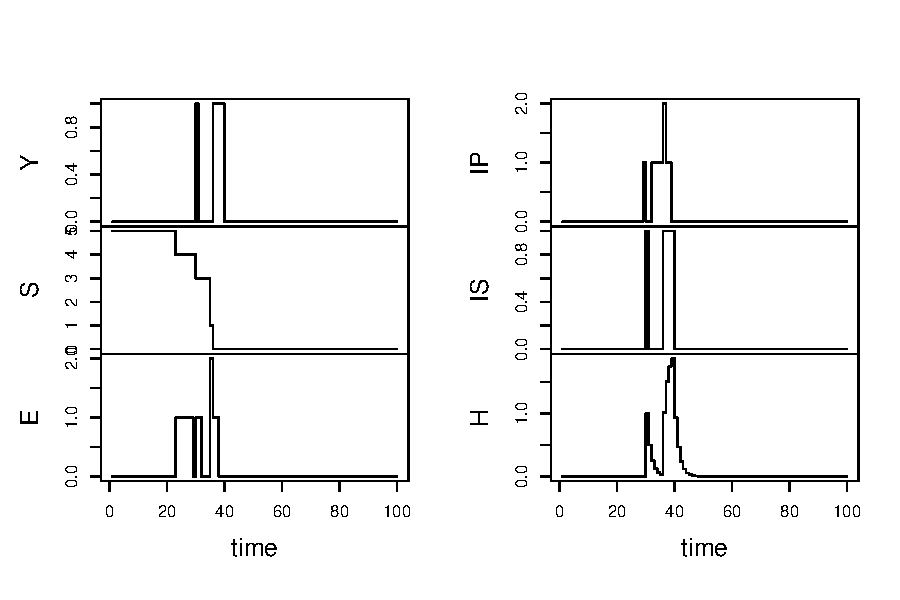
\includegraphics[width=\textwidth]{Images/SEIIR_traj.pdf}
\end{frame}

\begin{frame}{Méthodes particulaires}
Filtre à particules (SMC) permet de calculer \(\mathcal{L}(Y|\theta)\) par
simulation (méthode \emph{plug-and-play})
\begin{itemize}
\item Maximum de vraisemblance: filtrage itéré (Ionides et al. 2006, 2015)
\begin{itemize}
\item Marche aléatoire \(\theta_n\) pour les \(\theta\), variance \(\sigma_n\)
variable
\item \`A chaque itération, calcul de \(\mathcal{L}(Y|\theta_n)\) par SMC
\item \(\theta_n\to 0\) : convergence vers EMV \(\hat\theta_n\) sous conditions
de régularité du modèle
\item Implémentation R : paquet \texttt{pomp}
\end{itemize}
\item Estimation bayésienne: MCMC particulaire (Doucet et al. 2010)
\begin{itemize}
\item Utilise le filtre à particules comme moyen de calcul de la vraisemblance
dans un MCMC classique
\item Permet \emph{théoriquement} de faire de la sélection bayésienne de modèles
\item Plusieurs implémentations: \texttt{pomp} (R), LibBi (C++)
\end{itemize}
\end{itemize}
Méthodes très intensives en temps de calcul, surtout s'il faut considérer un
grand nombre d'observations indépendantes (N>10,000?)
\end{frame}

\end{document}
